\documentclass[8pt,xcolor=table]{beamer}

\usepackage{graphicx}
\usepackage{caption}
\usepackage{subcaption}
\usepackage{transparent}
 
% \usepackage[utf8]{inputenc}
% \usepackage[T1]{fontenc}
\usepackage[table]{xcolor}    % loads also »colortbl« 
%  \usepackage{enumitem}
% \usepackage{ucltemplate}
\usepackage{color}

\usepackage{tabularx} % make width of table columns evenly distributed (see http://tex.stackexchange.com/questions/60601/evenly-distributing-column-widths)
% \newcolumntype{Y}{>{\centering\arraybackslash}X}

% make entire row bold or italic in table
\newcommand\setrow[1]{\gdef\rowmac{#1}#1\ignorespaces}
\newcommand\clearrow{\global\let\rowmac\relax}
\clearrow


\usepackage{amssymb}% http://ctan.org/pkg/amssymb
\usepackage{pifont}% http://ctan.org/pkg/pifont
\newcommand{\cmark}{\ding{51}}%
\newcommand{\xmark}{\ding{55}}%


\usepackage{pgfgantt} % for grantt charts
\usepackage{rotating}
\usepackage[graphicx]{realboxes}
\usepackage[export]{adjustbox}
\usepackage{array}

\usepackage{rotating}
% \usepackage{tabularx, booktabs} % make width of table columns evenly distributed (see http://tex.stackexchange.com/questions/60601/evenly-distributing-column-widths)
% \newcolumntype{Y}{>{\centering\arraybackslash}X}

\DeclareMathOperator*{\argmin}{arg\,min}
\DeclareMathOperator*{\argmax}{arg\,max}

\usepackage{tikz}
\usetikzlibrary{arrows,positioning, shapes.symbols,shapes.callouts,patterns,shapes,chains,calc,backgrounds,fadings}

% \definecolor{parCol}{rgb}{0.1, 0.1, 1}
% \definecolor{stCol}{rgb}{0.1, 0.6, 0.1}
% \definecolor{bothCol}{rgb}{0, 0.5, 0.5}

\definecolor{parCol}{rgb}{0, 0, 0}
\definecolor{stCol}{rgb}{0, 0, 0}
\definecolor{bothCol}{rgb}{0, 0, 0}
\definecolor{blue3}{HTML}{86B7FC} % med blue
\definecolor{blue1}{HTML}{B5F1FF} % light blue
\definecolor{blue2}{HTML}{E0F9FF} % very light blue

\newcolumntype{C}[1]{>{\centering\let\newline\\\arraybackslash\hspace{0pt}}m{#1}}

\setlength{\tabcolsep}{0.2em}

 
 %% PRESENTATION FOR BOSTON VISIT %%
 
%Information to be included in the title page:
\title{TADPOLE Competition: Prediction of Alzheimer's Evolution using Statistical Models and Machine Learning}
\author[Raz \and Danny \and Seb]{
R\u{a}zvan Valentin Marinescu\vspace{1em} \and Leon Aksman
}

\institute{\small{Centre for Medical Image Computing, University College London, UK}

\vspace{0em}
}
\date{}

% logo of my university
\titlegraphic{
   \begin{figure}
   \begin{subfigure}{0.32\textwidth}
   \hspace{2em}
   \includegraphics[height=1.0cm]{../epsrc_logo.jpg}
   \end{subfigure}
   \begin{subfigure}{0.32\textwidth}
   \centering
   \includegraphics[height=1.5cm]{../NEWpond2017b.png} 
   \end{subfigure}
   \begin{subfigure}{0.32\textwidth}
   \centering
   \includegraphics[height=1.0cm]{../pondLogo.png} 
   \end{subfigure}
   \end{figure}
}

\setbeamercolor{frametitle}{fg=black}
\setbeamercolor{author in head/foot}{fg=black, bg=white} 
\setbeamercolor{institute in head/foot}{fg=black, bg=white} 
\setbeamercolor{title in head/foot}{fg=black, bg=white}
\setbeamercolor{date in head/foot}{fg=black, bg=white}

\setbeamersize{text margin left=10pt,text margin right=10pt}
% \setbeamertemplate{frametitle}{
%     \vspace{0.9em}
%     \insertframetitle
% %     \vspace{-3em}
% }
\setbeamertemplate{frametitle}{%
    \vspace{0.5em}
    \usebeamerfont{frametitle}\insertframetitle%
    \vphantom{g}% To avoid fluctuations per frame
    %\hrule% Uncomment to see desired effect, without a full-width hrule
    \par% <-- added
    \hspace*{-\dimexpr0.5\paperwidth-0.5\textwidth}% <-- calculation of left margin width
    \rule[0.5\baselineskip]{\paperwidth}{0.4pt}%
}

\setbeamertemplate{footline}
{
  \vspace{-3em}
  \leavevmode%
   \rule{\paperwidth}{0.3pt}
  \hbox{%
  \begin{beamercolorbox}[wd=.2\paperwidth,ht=2.25ex,dp=1ex,center]{author in head/foot}%
    \usebeamerfont{author in head/foot}Razvan V. Marinescu
  \end{beamercolorbox}%
  \begin{beamercolorbox}[wd=.3\paperwidth,ht=2.25ex,dp=1ex,center]{institute in head/foot}%
    \usebeamerfont{institute in head/foot} Leon Aksman
  \end{beamercolorbox}%
  \begin{beamercolorbox}[wd=.2\paperwidth,ht=2.25ex,dp=1ex,center]{institute in head/foot}%
    \usebeamerfont{institute in head/foot}University College London
  \end{beamercolorbox}%
  \begin{beamercolorbox}[wd=.2\paperwidth,ht=2.25ex,dp=1ex,center]{title in head/foot}%
    \usebeamerfont{title in head/foot}\insertsection
  \end{beamercolorbox}%
  \begin{beamercolorbox}[wd=.10\paperwidth,ht=2.25ex,dp=1ex,right]{date in head/foot}%
    \usebeamerfont{date in head/foot}\insertshortdate{}\hspace*{2em}
    \insertframenumber{} / \inserttotalframenumber\hspace*{2ex} 
  \end{beamercolorbox}}%
  \vskip0pt%
}

% \usepackage{beamerthemesplit}

\newcommand{\backupbegin}{
   \newcounter{finalframe}
   \setcounter{finalframe}{\value{framenumber}}
}
\newcommand{\backupend}{
   \setcounter{framenumber}{\value{finalframe}}
}


\makeatletter
\long\def\beamer@author[#1]#2{%
  \def\and{\tabularnewline}
  \def\insertauthor{\def\inst{\beamer@insttitle}\def\and{\tabularnewline}%
  \begin{tabular}{rl}#2\end{tabular}}%
  \def\beamer@shortauthor{#1}%
  \ifbeamer@autopdfinfo%
    \def\beamer@andstripped{}%
    \beamer@stripands#1 \and\relax
    {\let\inst=\@gobble\let\thanks=\@gobble\def\and{, }\hypersetup{pdfauthor={\beamer@andstripped}}}
  \fi%
}
\makeatother
\beamertemplatenavigationsymbolsempty
\setbeamertemplate{caption}[numbered]
\setbeamercolor{caption name}{fg=black}
\setbeamercolor{itemize item}{fg=black}
\setbeamercolor{itemize subitem}{fg=black}
\setbeamercolor{enumerate item}{fg=black}
\setbeamercolor{enumerate subitem}{fg=black}
\setbeamertemplate{enumerate item}[default]
\setbeamertemplate{enumerate subitem}[default]
\begin{document}
 
\section{Introduction}

\frame{\titlepage}
 
\setbeamerfont{frametitle}{size=\large}



\begin{frame}
\frametitle{Progression of Neurodegenerative Diseases (POND)}

\begin{figure}
\centering
\includegraphics[height=8cm]{../pond_diagram} 
\end{figure}

\end{frame}


\begin{frame}
\frametitle{POND Aim: Develop Computational Models for Disease Progression}

\newcommand{\mnpHeight}{3cm}

\vspace{-3em}
% \textbf{Background}:
% \onslide<1> \begin{itemize}
%   \item Aim: Develop computational models for disease progression
  
%   \vfill 
  
  \hspace{-2em}
  \begin{small}
  \begin{figure}[h]
  \centering
    \begin{minipage}[t][\mnpHeight][t]{0.49\linewidth}
  \centering
    \textbf{Event-Based Model}\\ \footnotesize{(Fontejin et al., Neuroimage, 2012)}\\    
    \includegraphics[width=0.9\textwidth,trim=0 0 0 0,clip]{../ebm_openday}
      \vspace{1em}
%     \includegraphics[width=0.4\textwidth]{young_positional_variance}
  \end{minipage}
  \begin{minipage}[t][\mnpHeight][t]{0.49\linewidth}
    \centering
    \textbf{Differential Equation Model}\\ \footnotesize{(Oxtoby et al., submitted, 2017)}
    \includegraphics[width=0.9\textwidth,trim=0 0 0 0, clip]{../dem_neil}
  \end{minipage}

  \vspace{2em}
  \begin{minipage}[t][\mnpHeight][t]{0.49\linewidth}
    \centering
    \textbf{Gaussian-Process Regression}\\ \footnotesize{(Lorenzi et al., IPMI, 2015)}
    \includegraphics[width=0.9\textwidth,trim=0 0 0 0, clip]{../lorenzi_ipmi2015}
    
    \vspace{2em}
    
  \end{minipage}
  \begin{minipage}[t][\mnpHeight][t]{0.49\linewidth}
    \centering
    \textbf{Subtype and Stage Inference}\\ \footnotesize{(Young et al., submitted, 2017)}
    \includegraphics[width=0.9\textwidth]{../sustain}
  \end{minipage}


  \end{figure}
  \end{small}
  
  \vspace{-2em}
  
% \end{itemize}


\end{frame}



\begin{frame}
\frametitle{POND Aim 2: Apply the Models to Distinct Neurodegenerative Diseases}

\newcommand{\mnpHeight}{3cm}

\vspace{-3em}
% \textbf{Background}:
% \begin{itemize}
%   \item 
  
%   \vfill 
  
  \hspace{-2em}
  \begin{small}
  \begin{figure}[h]
  \centering
  
      \begin{minipage}[t][\mnpHeight][t]{0.49\linewidth}
    \centering
    \textbf{typical AD}\\ \footnotesize{(Young et al., submitted, 2017)}
    \includegraphics[width=0.9\textwidth]{../young_progression.png}
  \end{minipage}
  \begin{minipage}[t][\mnpHeight][t]{0.49\linewidth}
    \centering
    \textbf{Familial AD}\\ \footnotesize{(Oxtoby et al., submitted, 2017)}
    \includegraphics[width=0.7\textwidth,trim=0 0 0 0, clip]{../neil_dian.png}
    
    \vspace{2em}
    
  \end{minipage}
  \vspace{2em}
  
    \begin{minipage}[t][\mnpHeight][t]{0.49\linewidth}
  \centering
    \textbf{Multiple sclerosis}\\ \footnotesize{(Eshaghi et al., Brain, 2017)}\\    
    \includegraphics[width=0.9\textwidth,trim=0 0 0 0,clip]{../ms_arman}
      \vspace{1em}
%     \includegraphics[width=0.4\textwidth]{young_positional_variance}
  \end{minipage}
  \begin{minipage}[t][\mnpHeight][t]{0.49\linewidth}
    \centering
    \textbf{Huntington's disease}\\ \footnotesize{(Wijeratne et al., in preparation)}
    \includegraphics[width=0.9\textwidth,trim=0 0 0 0, clip]{../hd_peter}
  \end{minipage}

\end{figure}
  \end{small}
  
%   \vspace{-2em}
  
% \end{itemize}

\end{frame}


\newcommand{\titleHigh}[1]{{\transparent{1.0}\textbf{#1}}} % title highlighting
\newcommand{\titleHighTwo}[1]{\underline{\textbf{#1}}} % title highlighting 2
\newcommand{\transpLevel}{0.4}

% \begin{frame}
% \frametitle{\textcolor{red}{Disease Progression} \textcolor{green}{Modelling} of \textcolor{blue}{Alzheimer's Disease} \textcolor{orange}{Subtypes}}
% 
% Title breakdown:\\
% \vspace{1em}
% \large{
% \textcolor{red}{Disease Progression} \textcolor{green}{Modelling} of \titleHighTwo{\textcolor{blue}{Alzheimer's Disease}} \textcolor{orange}{Subtypes}
% }
% 
% \vfill
% \vfill
% \vfill
% 
% \end{frame}



\begin{frame}
\frametitle{Alzheimer's Disease is a Devastating Disease}

\vspace{-1em}
\begin{itemize}
 \item 46 million people affected worldwide
 
  \begin{figure}
 \centering
%   \includegraphics[height=3cm]{adPrelavence}
  \includegraphics[height=4cm]{../adPrevalanceIncreasing}
 \end{figure}
 
 \onslide<2-> \item No treatments available that stop or slow down cognitive decline
 \onslide<2-> \item Q: Why did clinical trials fail? A: Treatments were not administered early enough 
 \vspace{1em}
 \onslide<3-> \item Q: How can we then identify subjects \textbf{early} in order to administer treatments? 
 \onslide<3-> \item A: Biomarkers ...
 


 
%  \item Many known AD biomarkers:
% 
% 
% % \vspace{-1em}
% \begin{figure}
% \centering
% 
% \begin{subfigure}{0.31\textwidth}
% \centering
% Cognitive tests\\
% \includegraphics[height=2cm]{cogAssessment}
% \end{subfigure}
% \begin{subfigure}{0.31\textwidth}
% \centering
% Atrophy (MRI)\\
% \includegraphics[height=2cm]{seeley_2009_topleft.png}
% \end{subfigure}
% \begin{subfigure}{0.31\textwidth}
% \centering
% % \vspace{1em}
% Hypometabolism (FDG PET)\\
% \includegraphics[height=2cm]{brainFDG}
% \end{subfigure}
% 
% 
% \vspace{1em}
% \begin{subfigure}{0.47\textwidth}
% \centering
% Tau aggregation (CSF, AV1451 PET)\\
% 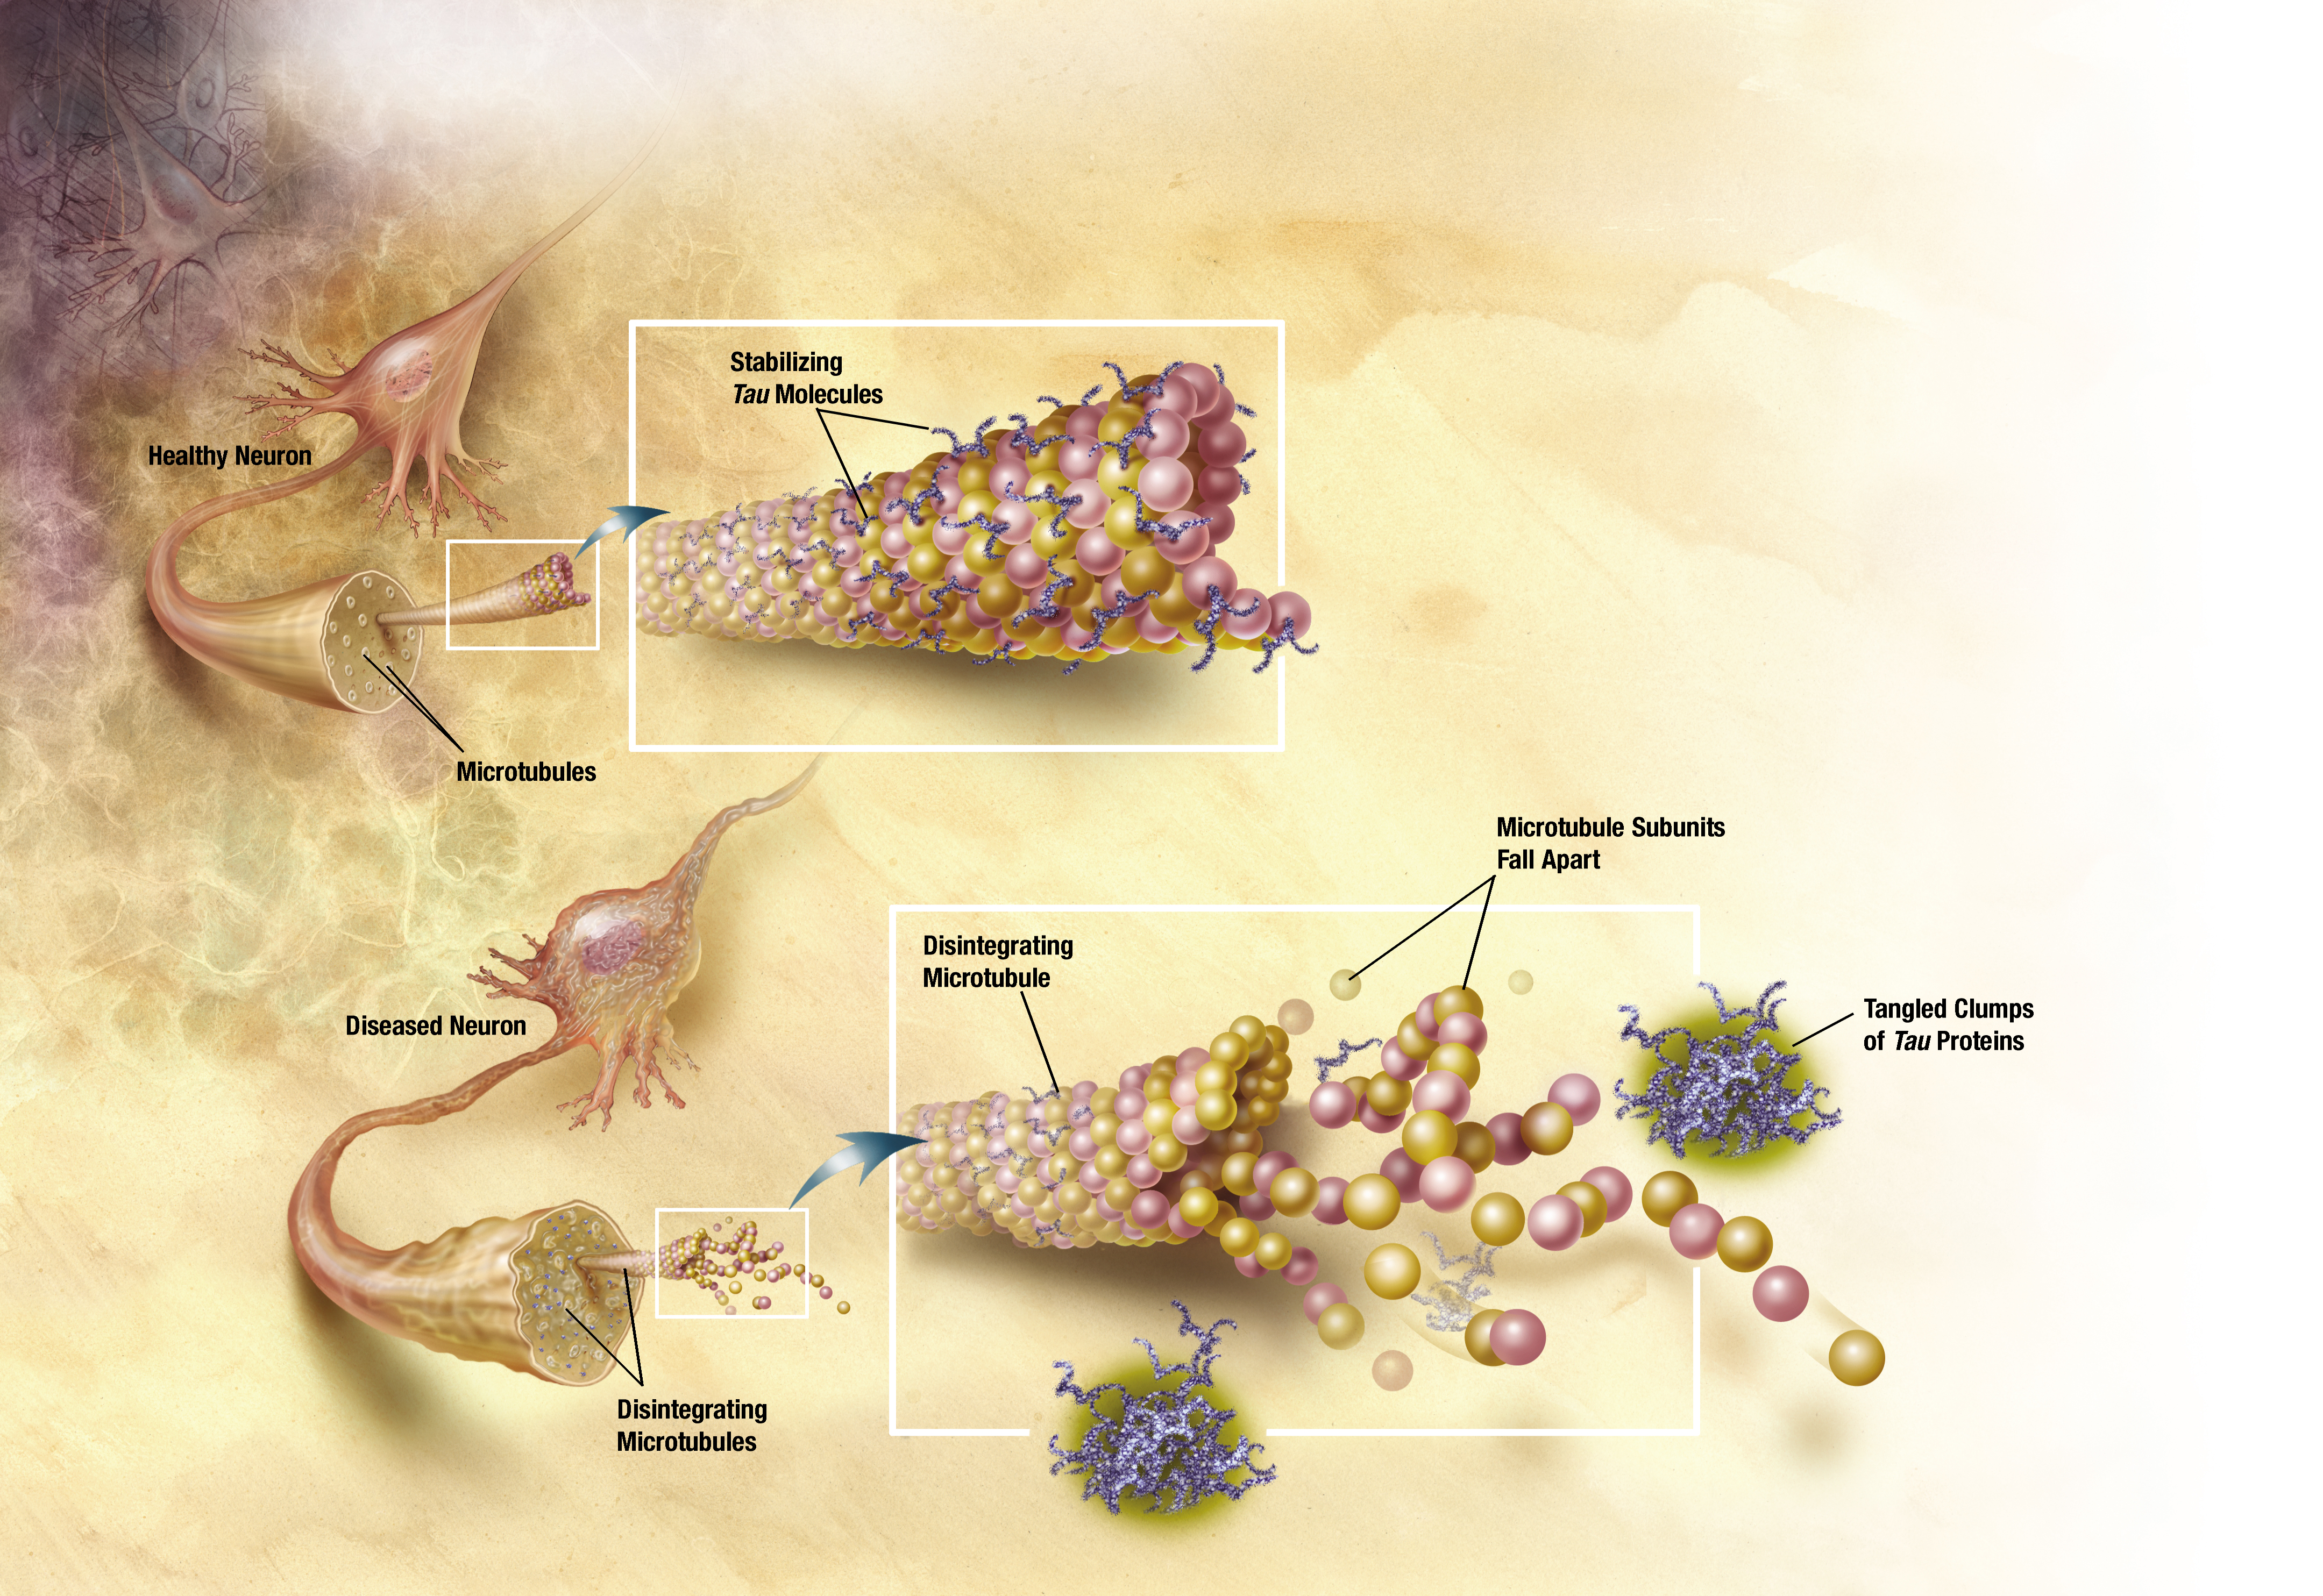
\includegraphics[height=2cm]{TANGLES_HIGH.jpg}
% \end{subfigure}
% \begin{subfigure}{0.47\textwidth}
% \centering
% % \vspace{1em}
% Amyloid misfolding (CSF, AV45 PET)\\
% \includegraphics[height=2cm]{amyloid_beta.png}
% \end{subfigure}
% 
% 
% 
% 
% \end{figure}



\end{itemize}

\vspace{-1em}

\end{frame}

% Also say that we cannot build the model on age
\begin{frame}
\frametitle{Biomarker Evolution creates a Unique Disease Signature\\
that can be used for Staging Individuals in Clinical Trials}
% explain what are the challenges

\begin{figure}
\centering 
\vspace{1em}
\includegraphics[height=5cm]{../adniDiseaseProgression}
\hspace{-4em}ADNI website 

\end{figure}


\begin{itemize}
 \item Accurate disease staging $\rightarrow$ better patient stratification
 \item Problem: This is a "hypothetical" (i.e. qualitative) disease progression model
 \item Why construct a quantitative model? 
\end{itemize}

\end{frame}


\section{Disease Progression Modelling}

% \begin{frame}
% \frametitle{\textcolor{red}{Disease Progression} \textcolor{green}{Modelling} of \textcolor{blue}{Alzheimer's Disease} \textcolor{orange}{Subtypes}}
% 
% Title breakdown:\\
% \vspace{1em}
% \large{
% \titleHighTwo{\textcolor{red}{Disease Progression} \textcolor{green}{Modelling}} of \textcolor{blue}{Alzheimer's Disease} \textcolor{orange}{Subtypes}
% }
% 
% \vfill
% \vfill
% \vfill
% 
% \end{frame}

\begin{frame}
\frametitle{Benefits of Quantitative Disease Progression Models}

\begin{overprint}
 \onslide<1>\begin{figure}
 \centering
\includegraphics[height=5cm,trim=0 0 650 0,clip]{../dpmDiffDiag1.png}
\end{figure}

\onslide<2> \begin{figure}
 \centering
\includegraphics[height=5cm,trim=0 0 650 0,clip]{../dpmDiffDiag2.png}
\end{figure}

\onslide<3-> \begin{figure}
 \centering
\includegraphics[height=5cm,trim=0 0 0 0,clip]{../dpmDiffDiag2.png}
\end{figure}

\end{overprint}

\vspace{1em}
\begin{itemize}
 \onslide<1-> \item Basic biological insight
 \onslide<2-> \item Staging can help stratification in clinical trials
 \onslide<3-> \item Differential diagnosis and prognosis
 \onslide<4-> \item Predict future evolution of patients
 \onslide<5-> \item Early detection of disease in at-risk subjects
 
 
 \vspace{1em}
 \onslide<6-> \item[] \textbf{Need to identify which models and features are best at above tasks ...}
 \vspace{1em}
\end{itemize}


 

\end{frame}



\section{TADPOLE}

\begin{frame}
\frametitle{TADPOLE Challenge aims to identify algorithms that best predict future evolution of subjects at-risk of AD}

\vspace{-3em}
\begin{figure}[H]
\centering
\includegraphics[height=3.5cm]{../tadpole_diagram} 
\end{figure}

\begin{figure}[H]
\centering
\includegraphics[height=1.2cm]{../../upgrade_report/epsrcPres/tadpole} 
\end{figure}

\footnotesize{TADPOLE Challenge: Prediction of Longitudinal Evolution in Alzheimer's Disease\\
Razvan V. Marinescu, Neil P. Oxtoby, Alexandra L. Young, Esther E. Bron, Arthur W. Toga, Michael W. Weiner, Frederik Barkhof, Nick C. Fox, Stefan Klein, Daniel C. Alexander, the EuroPOND Consortium, arXiv, 2018} 

\end{frame}

\begin{frame}
\frametitle{What to do}

% My work on the challenge:
\begin{columns}[T]
\begin{column}{.55\textwidth}
\textbf{Input}: Large dataset from ADNI:
\begin{itemize}
 \item $>$ 1,667 subjects with a total of 12,000 visits.
 \item $>$ 2,000 biomarkers from imaging, demographic, cognitive and genetic data
\end{itemize}

\vspace{8em}

\textbf{Task}: Estimate the pregression over the next 5 years of three key biomarkers:
\begin{itemize}
 \item Diagnosis   
 \item ADAS-COG13
 \item Ventricle Volume
\end{itemize}

\end{column}
\begin{column}{.45\textwidth}
\begin{figure}
 \centering
 \vspace{-2em}
\includegraphics[width=0.8\textwidth]{../tadpole_data_types}

\end{figure}

\end{column}
\end{columns}

\vspace{-6em}
\begin{figure}[H]
% \right
\includegraphics[width=0.75\textwidth,right]{forecasts_table} 
\end{figure}

\end{frame}


\begin{frame}
\frametitle{Evaluation}


% \textbf{Task}: Score as high as possible on the following three criteria:
% 
% 
% \vfill

\textbf{Overall winner}: lowest sum of ranks in the three categories above
\begin{itemize}
 \item Diagnosis MAUC
 \item ADAS-COG13 MAE
 \item Ventricle Volume MAE
\end{itemize}

\vfill

We will offer prizes!

\vfill

\textbf{Live leaderboard} will show progress of each team this week:
\begin{figure}
\centering
\includegraphics[height=4cm]{../leaderboard} 
\end{figure}

\end{frame}


\begin{frame}
\frametitle{Join the TADPOLE Challenge!}

\begin{itemize}
 \item URL: https://tadpole.grand-challenge.org/
 \item Prize fund: \pounds 30,000
\end{itemize}

\begin{figure}
\centering
\includegraphics[scale=0.4,trim=0 270 0 0,clip]{../tadpole} 
\end{figure}


\end{frame}


\end{document}



